\documentclass{beamer}
\usepackage[utf8]{inputenc}
\usepackage[brazil]{babel}
\usepackage{xcolor}
\usepackage{tikz}
\usetikzlibrary{positioning,calc}
\usepackage{graphicx}
\usepackage{cite}
\usepackage{hyperref}
\usepackage{array}
\usepackage{amsmath}
\usepackage{amssymb}
\usepackage{amsthm}
\usepackage{listings}
\usepackage{fontawesome}
\usepackage{caption}
\usepackage{subcaption}
\usepackage{wrapfig}
\usetheme{mtmufsc} %%%%%%%%Use this template
\renewcommand{\qedsymbol}{$\blacksquare$}
\usepackage[alf]{abntex2cite}


% This is a beamer template inspired by unofficial Oxford University Beamer Template, made by Clara Eleonore Pavillet.
\title{O poder da Aprendizagem Profunda}
\author{Felipe Kaminsky Riffel}
\date{\today}
\institute{Universidade Federal de Santa Catarina}

\begin{document}

{\setbeamertemplate{footline}{} 
\frame{\titlepage}}
% \frame{}

\begin{frame}{Sumário}
    \tableofcontents
\end{frame}
  
% %Sempre que iniciar uma nova sessão, você pode fazer um slide de transição com o índice.
% \begin{frame}
% \tableofcontents[currentsection]
% \end{frame}

\section{Artigo: Why does deep and cheap learning work so well?}    
\begin{frame}
\tableofcontents[currentsection]
\end{frame}

\begin{frame}{Why does deep and cheap learning work so well?}

Artigo: \\

LIN, Henry W.; TEGMARK, Max; ROLNICK, David. Why does deep and cheap learning work so well? Journal of Statistical Physics, v. 168, n. 6, p. 1223–1247, 2017.

\end{frame}

\subsection{Introdução}
\begin{frame}
    \tableofcontents[currentsection]
\end{frame}


\begin{frame}{Introdução}

Três problemas principais da teoria de redes neurais: \\

\begin{itemize}
    \item Expressabilidade: que funções podemos expressar? \pause \\
    \item Eficiência: quão complexa a rede tem que ser? \pause \\
    \item "Aprendibilidade": quão rápido a rede consegue aprender a ajustar os bons parâmetros? \footnote[frame]{Traduzido de "Learnability"} \pause
\end{itemize}

Aqui, focamos nos dois primeiros: \textbf{Expressabilidade} e \textbf{Eficiência}.
\end{frame} 

\begin{frame}{Introdução}
    Problema: "como redes neurais funcionam bem na prática, se o número de funções possíveis é exponencialmente maior que o número de redes possíveis?"

\end{frame}


\begin{frame}{Introdução}

    \textbf{Exemplo:} imagem preta/branca de 1MP ~ vetor de 1000000 entradas com 256 valores possíveis (valor em cada pixel)

    \pause

    \begin{columns}
        \begin{column}{0.3\textwidth}
            \begin{figure}
                
\includegraphics[width=\textwidth]{fig/keyboard-cat.png}
            \end{figure}
        \end{column}
        \begin{column}{0.1\textwidth}
            \[
                \iff
            \]
        \end{column}
        \begin{column}{0.3\textwidth}
            \small
            \[
                \begin{pmatrix}
                    x_1 \\
                    \vdots \\
                    x_{1000000}
                \end{pmatrix}
            \]
            \[
            x_i \in I_{256} := \{1,2,3,\dots,256\}
            \]
        \end{column}
    \end{columns}

    \pause

    \vspace{1em}

    Nº total de imagens possíveis: $256^{1000000}$.

    \pause
    \vspace{1em}

    Se existe $p: I_{256} \to (0,1)$ que associa cada imagem a uma probabilidade, p deve ter uma lista $256^{1000000}$ valores (!!!)
\end{frame}

\begin{frame}
    Porém, redes neurais relativamente simples conseguem calcular bem a tarefa.
    
    \small

    \begin{columns}
        \begin{column}{0.3\textwidth}
            \begin{figure}
                
\includegraphics[width=\textwidth]{fig/keyboard-cat.png}
            \end{figure}
        \end{column}
        \begin{column}{0.3\textwidth}
            \begin{figure}
                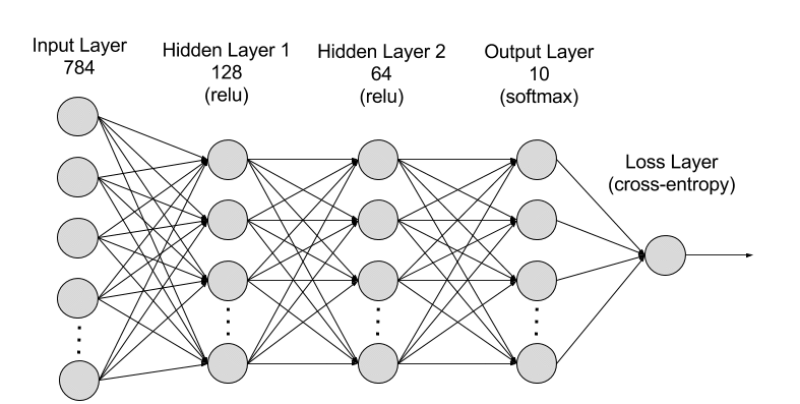
\includegraphics[width=\textwidth]{fig/nn.png}
            \end{figure}
        \end{column}
        \begin{column}{0.3\textwidth}
            \[
                p(\text{Gato} |\bf{x}) = 83\%
            \]
        \end{column}
    \end{columns}
    
    \vspace{1em}

    \pause

    A \textbf{matemática} ajuda a explicar: as redes neurais conseguem diminuir drasticamente a explosão combinatória de número de parâmetros em relação ao número de valores;
    \vspace{1em}
    
    \pause

    A razão também é \textbf{física}: as leis sugerem que os datasets de interesse são, em sua maioria, advindos de distribuições simples.

\end{frame}


\subsection{Expressabilidade e Eficiência de Redes Rasas}
\begin{frame}
    \tableofcontents[currentsection]
\end{frame}

\begin{frame}{Redes neurais}

    Considere $\mathbf x \in \mathbb R^d$. Sejam $A_i:\mathbb R^d \to \mathbb R^d$ operadores afim, i.e.,

    \[
        A_i = W_i - b_i
    \]
    com $W_i \in \mathbb R^{m_i \times n_i}$ e $b_i \in \mathbb R^{n_i}$.

    \vspace{1em}

    \pause 

    Dadas $\sigma_i:\mathbb R^{m_i} \to \mathbb R^{m_i}$ não linear, chamamos de rede neural feedforward uma função $\mathbf f: \mathbb R^n \to \mathbb R^m$ da forma:

    \begin{equation}
        \mathbf f (\mathbf x) = \sigma_k A_k \dots \sigma_2 A_2 \sigma_1 A_1 \mathbf x.
    \end{equation}

    \pause 

    \begin{itemize}
        \item Aqui, se admite também $\sigma_k = I$; 
        \item Cada composição $\sigma_i A_i$ é chamada de \textit{camada} da rede;
        \item Cada componente da operação $\sigma_{ij} A_{i,j} x$ (linha da matriz + aplicação de $\sigma_i$) é chamado de \textit{neurônio};
    \end{itemize}

\end{frame}

\begin{frame}{Redes neurais}
    $\mathbf \sigma_i$ pode ser qualquer operador não linear. Escolhas comuns são, dado $\mathbf x = (x_1, \dots, x_n)$:

    \begin{itemize}
        \item Função local: escolha $\sigma : \mathbb R \to \mathbb R$ não linear e aplique ponto a ponto $\mathbf \sigma_i(\mathbf x) = (\sigma(x_1),\dots,\sigma(x_n))$; \pause \\
        \item Max-pooling: $\sigma_i (\mathbf x) = \max_{j=1,\dots,n} (x_j)$; \pause \\
        \item Softmax: \[
            \sigma_i(\mathbf x) = \frac{1}{\sum_{j=1}^n e^{x_j}}(e^{x_1}, \dots, e^{x_n}). 
        \]
    \end{itemize}

\end{frame}

\begin{frame}{Teorema 1 (Aproximação da multiplicação)}
    Seja $\mathbf f$ rede neural da forma $\mathbf f (\mathbf x) = A_2 \sigma A_1\mathbf x$, onde $\mathbf \sigma$ é aplicação não linear ponto a ponto qualquer. Considere as camadas de entrada, escondida e de saída com tamanhos 2, 4 e 1 respectivamente. Então, $\mathbf f$ pode aproximar uma porta de multiplicação arbitrariamente bem.

    Ou seja, dado $\varepsilon>0$, para qualquer $\sigma$ não linear (aplicada ponto a ponto), existem  $A_1:\mathbb R^2 \to \mathbb R^4, A_2:\mathbb R^4 \to \mathbb R$ tais que a rede $f(x) = A_2 \sigma A_1 \mathbf{x}$ é tal que, dado $x=(u \; v)^T$ qualquer

    \[
        |f(x) - uv|<\varepsilon
    \]

    para $u,v$ em um compacto qualquer.

\end{frame}

\begin{frame}{Teorema 1 - Demonstração}
    \small
    Seja $\sigma:\mathbb R \to \mathbb R$ não linear qualquer suficientemente suave. Na expansão de Taylor em torno de $x=0$:

    \[
        \sigma(u) = \sigma(0) + \sigma'(0)u + \frac{u^2}{2} \sigma''(0) + \mathcal O(u^3).
    \]

    Sem perda de generalidade, considere $\sigma''(0) \neq 0$ (ou então, ajuste $b_1$ para que $\sigma''(A_{1,1}x-b_{1,1}),\sigma''(A_{1,2}x-b_{1,2})\neq0$, que deve existir dado que é não linear). 

    \vspace{1em}
    \pause

    Então,

    \begin{align*}
        m(u,v) &:= \frac{\sigma(u+v)+\sigma(-u-v)-\sigma(u-v)-\sigma(v-u)}{4\sigma''(0)} \\ 
        &= \sigma''(0) \frac{(u+v)^2 + (-u-v)^2 - (u-v)^2 - (v-u)^2  + \mathcal O((u+v)^3)}{4\sigma''(0)}  \\
        &= uv + \mathcal O((u+v)^3)
    \end{align*}
\end{frame}


\begin{frame}{Teorema 1 - Demonstração}
    Ou seja, $m(u,v) = uv + \mathcal O((u+v)^3)$, de modo que $\lim_{u^2+v^2 \to 0} \frac{m(u,v)-uv}{u^2+v^2} = 0$. 
    
    \pause

    Veja que, $m(u,v) = A_2 \sigma A_1 (u \; v)^T$, onde:

    \begin{equation*}
        A_1 = W_1 - b_1= \begin{pmatrix}
            1 & 1 \\
            -1 & -1 \\
            1 & -1 \\
            -1 & 1
        \end{pmatrix} - b_1,
    \end{equation*}

    \begin{equation*}
        A_2 = W_2 = (4\sigma''(0))^{-1} \begin{pmatrix}
            1 & 1 & -1 & -1
        \end{pmatrix} -b_2.
    \end{equation*}

    \pause
    \vspace{1em}
\end{frame}

\begin{frame}{Teorema 1 - Demonstração}
    Taylor fornece uma estimativa local, sendo boa para $u,v \approx 0$. Para $u,v$ num compacto de raio qualquer, tome $ A_1 = \lambda W_1 - b_1$ e $A_2 = \lambda^{-2}W_2 - b_2$ na definição de $\mathbf f$, de modo a obter
    \begin{align*}
        f(x) = (\lambda^{-2}A_2)\sigma(\lambda A_1)x = \lambda^{-2} ( \lambda u \lambda v) = uv,
    \end{align*}
    tornando a estimativa tão boa quanto se queira. $\square$
\end{frame}

\begin{frame}{Teorema 1 - Comentário}
    \begin{figure}
        \caption{Ilustração da arquitetura da rede no teorema anterior}
        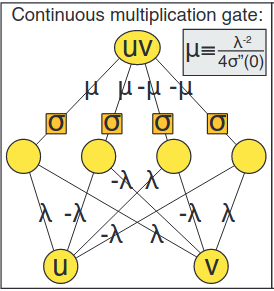
\includegraphics[width=0.5\textwidth]{fig/productgate.png}
        \caption*{Fonte: Lin, et.al. (2017)}
    \end{figure}
\end{frame}

\begin{frame}{Corolário 1}
    
    \textbf{Corolário}: Para cada polinômio multivariado e qualquer tolerância $\varepsilon>0$ existe uma rede neural de tamanho finito $N$ (independente de $\varepsilon$) que aproxima o polinômio a uma precisão melhor que $\varepsilon$. Além disso, $N$ é limitado pela complexidade do polinômio, escalando conforme o número de multiplicações requeridas vezes um fator ligeiramente maior que 4.
    
\end{frame}

\begin{frame}{Corolário - Demonstração (ideia)}
    \small
    Ideia: montamos uma rede neural em "blocos", onde cada produto pode ser representado por uma rede neural descrita no teorema anterior.
    
    \vspace{1em}

    Cada produto necessita de 4 neurônios de camada escondida (a saída de um neurônio corresponde à entrada do seguinte). Ainda, temos neurônios a mais para os termos remanescentes, fazendo a passagem de uma camada para a outra, sem alterar o valor. O número de passagens é 

    
    \pause 
    \vspace{1em}

    Para os termos remanescentes, podemos construir uma "camada de passagem" $u \mapsto u$ com 1 neurônio, dado que:

    \[
        u \approx \frac{\sigma(u) - \sigma(0)}{\sigma'(0)}
    \]
\end{frame}

\begin{frame}{Corolário 1 - Demonstração (ideia)}
    
    \begin{figure}
        \caption{Ilustração da rede construída: em \textcolor{red}{vermelho}, conexões de produto (4 neurônios); em \textcolor{blue}{azul}, camadas de passagem (1 neurônio)}.
        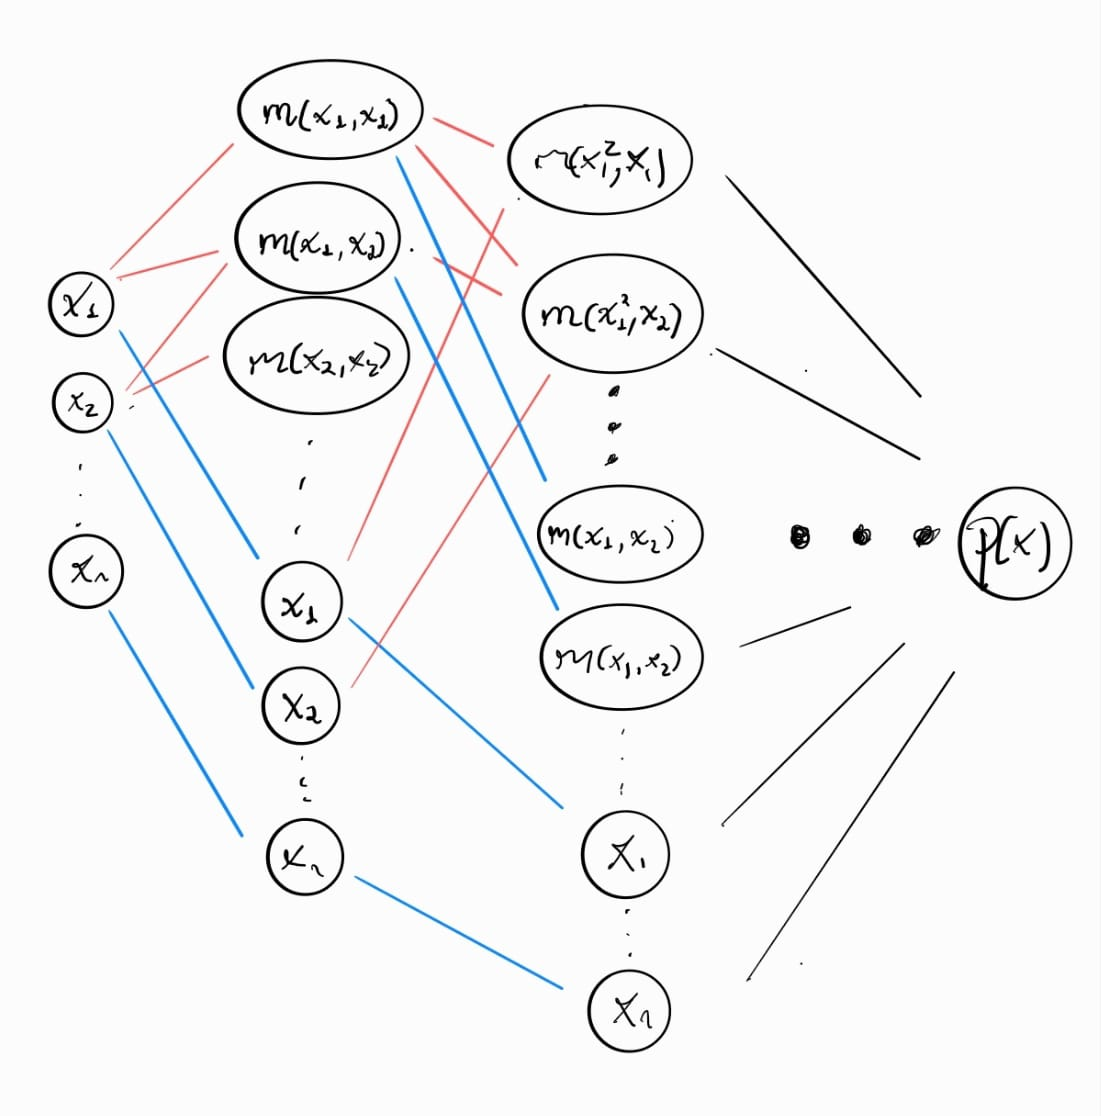
\includegraphics[width=0.5\textwidth]{fig/rede-corolario.jpeg}
        \caption*{Fonte: Autor.}
    \end{figure}

\end{frame}


\begin{frame}{Corolário - Demonstração}
    \small
    Dadas $n$ variáveis, conseguimos aproveitar cada camada anterior , pois para obter um polinômio:
    \begin{itemize}
        \item de grau 2, multiplicamos cada variável entre si e passamos as demais adiante, nos dando $4n^2 + n \leq 5n^2$ neurônios; \pause
        \item de grau 3, multiplicamos os $n^2$ termos de grau 2 por cada variável e passamos os termos restantes, nos dando $4n^3 + $; \pause
        \item $\vdots$ ; 
        \item de grau $d$, mutiplicamos os $n^{d-1}$ termos de grau $d-1$ entre as $n$ variáveis e passamos os demais adiante, tendo $4n^d + n^{d-1}+ \dots + n \leq 5n^d$ neurônios; \pause
    \end{itemize}

    No final, temos um número de neurônios da ordem de:
    \[
        5n^2 + 5n^3 + \dots + 5n^d = \mathcal O (5n^d).
    \]
\end{frame}

\begin{frame}{Corolário 1 - Comentário}
    Se $\mathbf x \in \{0,1\}^n $, temos $x_i^2 = x_i$, de modo que todo polinômio assume a forma

    \begin{equation*}
        p(\mathbf x) = a_0 + \sum_i a_{i} x_i + \sum_{i<j} a_{ij} x_{i}x_{j} + \sum_{i<j<k} a_{ijk} x_{i}x_{j}x_{k} \cdots 
    \end{equation*}

   No total, temos $2^n$ termos distintos.

    \vspace{1em}
\end{frame}

\begin{frame}{Corolário 1 - Comentário}
    \small
    \begin{columns}
        \begin{column}{0.6\textwidth}
            Ainda, qualquer produto de binários pode ser representado com um único neurônio na camada escondida com $\sigma(x) = \frac{1}{1+e^{-x}}$:
            \[
                \prod_{i \in K} x_i = \lim_{\beta \to \infty} \sigma \left[ -\beta \left( k - \frac{1}{2} - \sum_{i \in K} x_i \right) \right],
            \]
            pois $\sigma(x)\to 0$ se $x\to -\infty$ e $\sigma(x) \to 1$ se $x\to \infty$.
            
        \end{column}    
        \begin{column}{0.4\textwidth}
            \pause
            \begin{figure}
                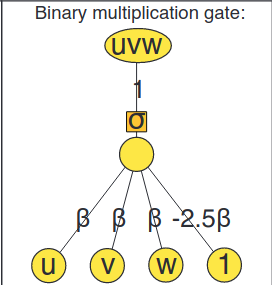
\includegraphics[width=0.9\textwidth]{fig/binproductgate.png}
            \end{figure}
        
        \end{column}
    \end{columns}

    
\end{frame}

\begin{frame}{Comentário}
    
    Assim, qualquer polinômio de $n$ variáveis binárias pode ser representado por uma rede com:

    \begin{itemize}
        \item Uma camada de entrada, com $n+1$ neurônios;
        \item Uma camada escondida, com $2^n$ neurônios (um para cada produto e termo livre);
        \item Uma camada de saída.
    \end{itemize}
 
\end{frame}

\subsection{Custos de Achatamento}
\begin{frame}
    \tableofcontents[currentsection]
\end{frame}

\begin{frame}{Custo de Achatamento}
    \textbf{Exemplo:} Fatoração de matrizes
    \begin{itemize}
        \item FFT (Transformada rápida de Fourier);
        \item Matrizes de posto baixo: $A = MN$, com $M_{n\times k}, N_{k \times n}$;
        \item Cholesky, LU, QR esparsas;  
    \end{itemize}
\end{frame}

\begin{frame}{Teorema 2}
    \textbf{Teorema:} Dados $x_1,\dots,x_n \in \mathbb R$ e $\sigma \in C^\infty$, o monômio $\Pi_{i=1}^n x_i$ pode ser aproximado por uma rede neural de 1 camada com $2^n$ neurônios, seguindo a fórmula

    \[
        \Pi_{i=1}^n x_i \approx \frac{1}{2^n} \sum_{\{s\}}s_1 \cdots s_n \sigma(s_1 x_1 + \cdots + s_n x_n),
    \]

    onde $s_i \in \{-1,1\}$, para cada $i = 1,\dots,k$, e a soma é tomada sobre todas as $2^n$ configurações possíveis de $s_1 \cdots s_n$.

    \pause

    Além disso, essa é a menor rede de 1 camada capaz de fazer tal aproximação.

\end{frame}

\begin{frame}{Teorema 2 - Demonstração}
    \small
    Dado $x = (x_1,x_2, \dots, x_n)$, uma rede $N$ de 1 camada escondida é da forma

    \[
        N(x) = \sum_{j=1}^m w_j \sigma \left(\sum_{i=1}^n a_{ij} x_i \right)
    \]

    \pause

    Queremos uma rede de tamanho $m$ com pesos $w_j$ e $a_{ij}$ tal que, denotando $\sigma_k = \sigma^(k)(0)$:
    
    \begin{equation} 
        \sigma_n \sum_{j=1}^{m} w_j \left( \sum_{i=1}^{n} a_{ij} x_i \right)^{n} = \prod_{i=1}^{n} x_i,
    \end{equation}
    
    \begin{equation}
        \sigma_k \sum_{j=1}^{m} w_j \left( \sum_{i=1}^{n} a_{ij} x_i \right)^{k} = 0, \forall k \in \{1, \dots, n-1\}
    \end{equation}

    \pause

    Mostremos que $m=2^n$ é necessário e suficiente.

\end{frame}

\begin{frame}{Teorema 2 - Demonstração}
    \textbf{$2^n$ Suficiente} Sejam $S_1,S_2, \dots, S_m$ subconjutos de $\{1,\dots,n\}$. Defina p/ cada $i\in \{1, \dots, n\}$
    \[
        s_i(S) = \begin{cases}
            -1, i \in S,\\
            1, i \notin S.
        \end{cases}
    \]
    \pause
    
    Defina $a_{ij} = s_i(S_j)$

    \[
        w_j =x \frac{1}{2^n n! \sigma_n} \prod_{i=1}^{n} a_{ij} = \frac{(-1)^{|S_j|}}{2^n n! \sigma_n}.
    \]

\end{frame}

\begin{frame}{Teorema 2 - Demonstração}
    
    Considere $p(x) = x_1^{r_1}x_2^{r_2}\cdots x_1^{r_1}, r_1+\cdots+r_n=r\leq n$. Vamos verificar que no desenvolvimento de 
    \[
        \sigma_r \sum_{j=1}^{m} w_j \left( \sum_{i=1}^{n} a_{ij} x_i \right)^{r}
    \]
    se $p(x) \neq \prod_i^n x_i$, seu coeficiente é 0.
\end{frame}

\begin{frame}{Teorema 2 - Demonstração}
    \small
    Se $p(x)\neq \prod_i^n x_i$, existe $r_{i_0}=0$.

    \begin{align}
        \sigma_r \sum_{j=1}^{m} w_j \left( \sum_{i=1}^{n} a_{ij} x_i \right)^{r} \\
        = \sigma_r \sum_{j=1}^{m} \frac{(-1)^{|S_j|}}{2^n n! \sigma_n} \left( \sum_{i=1}^{n} s_{i}(S_j) x_i \right)^{r}
    \end{align}
    \pause
    \[
        = \sigma_r \sum_{S_j \not \owns i_0}^{m} \left[ \frac{(-1)^{|S_j|}}{2^n n! \sigma_n} \left( \sum_{i=1}^{n} s_{i}(S_j) x_i \right)^{r} + \frac{(-1)^{|S_j \cup \{i_0\}|}}{2^n n! \sigma_n} \left( \sum_{i=1}^{n} s_{i}(S_j \cup \{i_0\}) x_i \right)^{r} \right]
    \]
    \pause
    \[
        = \sigma_r \frac{(-1)^{|S_j|}}{2^n n! \sigma_n} \sum_{S_j \not \owns i_0}^{m} \left[  \left( \sum_{i=1}^{n} s_{i}(S_j) x_i \right)^{r} - \left( \sum_{i=1}^{n} s_{i}(S_j \cup \{i_0\}) x_i \right)^{r} \right]
    \]
\end{frame}

\begin{frame}{Teorema 2 - Demonstração}
    Veja que $s_i(S_j) = s_i (S_j \cup \{i_0\}), \forall i \neq i_0$. Logo, se $r_{i_0}=0$ em $p(x)$, os coeficientes são iguais, portanto, se cancelam em
    \[
        \left( \sum_{i=1}^{n} s_{i}(S_j) x_i \right)^{r} - \left( \sum_{i=1}^{n} s_{i}(S_j \cup \{i_0\}) x_i \right)^{r} 
    \]
    \pause
    Isso vale para cada $i_0$. Em particular, para cada $r<n$, vale que:
    \[
        \sigma_r \sum_{j=1}^{m} w_j \left( \sum_{i=1}^{n} a_{ij} x_i \right)^{k} = 0,
    \]
    como queríamos;
\end{frame}


\begin{frame}{Teorema 2 - Demonstração}
    \small
    Se $p(x) = \prod x_i$, o coeficiente na expansão de $\left(\sum a_{ij} x_i \right)^n$ é 

    \[
        n! \prod_i a_{ij} = n! (-1)^{|S_j|}
    \]
    \pause
    Logo,
    \begin{align*}
        \sigma_n \sum_j^m w_j \left(\sum a_{ij} x_i \right)^n \\
        = \sigma_n \sum_j^{2^n} \frac{(-1)^{|S_j|}}{2^n n! \sigma_n} \left(\sum a_{ij} x_i\right)^n  \\
        = \sigma_n \sum_j^{2^n} \frac{(-1)^{|S_j|}}{2^n n! \sigma_n} n! (-1)^{|S_j|} = \prod_{i=1}^n x_i
    \end{align*}
    
    como queríamos.
\end{frame}


\begin{frame}{Teorema 2 - Demonstração}
    \textbf{$2^n$ é Necessário:} Suponha que existe uma rede de uma camada escondida com $m$ neurônios e pesos $w_j, a_{ij}$ que satisfaz as condições desejadas:
        
    \begin{equation*} 
        \sigma_n \sum_{j=1}^{m} w_j \left( \sum_{i=1}^{n} a_{ij} x_i \right)^{n} = \prod_{i=1}^{n} x_i,
    \end{equation*}
    
    \begin{equation*}
        \sigma_k \sum_{j=1}^{m} w_j \left( \sum_{i=1}^{n} a_{ij} x_i \right)^{k} = 0, \forall k \in \{1, \dots, n-1\}
    \end{equation*}

    Mostremos que $m\geq 2^n$.
\end{frame}

\begin{frame}{Teorema 2 - Demonstração}
    Seja $S \subset \{1,\dots,n\}$. Tomando todas as parciais $\frac{\partial }{\partial x_h}$ para $h\in S$ nas duas equações:

    \begin{equation} 
        \label{eq:partial-prod}
        \frac{n! \, \sigma_n}{|n - S|!} \sum_{j=1}^{m} w_j \prod_{h \in S} a_{hj} 
        \left( \sum_{i=1}^{n} a_{ij} x_i \right)^{n - |S|} = \prod_{h \notin S} x_h,
    \end{equation}

    \begin{equation}
        \label{eq:partial-zero}
        \frac{k! \, \sigma_k}{|k - S|!} \sum_{j=1}^{m} w_j \prod_{h \in S} a_{hj} 
        \left( \sum_{i=1}^{n} a_{ij} x_i \right)^{k - |S|} = 0, k \geq |S|
    \end{equation}    

\end{frame}

\begin{frame}{Teorema 2 - Demonstração}

    Sejam $S_1,\dots, S_{2^n}$ os subconjuntos de $\{1,\dots,n\}$ e defina $A \in \mathbb R^{2^n \times m}$ por 
    \[
        A_{ij} = \prod_{h \in S_i} a_{hj}.
    \]

    Ideia: mostrar que $A$ tem posto linha completo. 

    \pause
    Suponha por contradição que exista uma dependência linear nas linhas de $A$:
    \[
        c^T A = \sum_l^r c_l A_{l} = 0
    \] 
    com cada $S_l$ distinto entre si e $c_l \neq 0$, para cada $l$.
    Seja $s=\max_{\ell | \sum_l^r c_l A_{l} = 0} |S_\ell|$. 
    \pause
    Defina $d \in \mathbb R^m$ por 
    \[
        d_j = w_j\left( \sum_{i=1}^{n} a_{ij} x_{i} \right)^{n-s}.
    \]
\end{frame}

\begin{frame}{Teorema 2 - Demonstração}
    Então,
    \begin{equation*}
        0 \ = \ \mathbf{c}^{t} \mathbf{A} \mathbf{d} = \sum_{\ell=1}^{r} c_{\ell} \sum_{j=1}^{m} w_{j} \prod_{h \in S_{\ell}} a_{hj} \left( \sum_{i=1}^{n} a_{ij} x_{i} \right)^{n-s}
    \end{equation*}
    \pause
    \begin{equation*}
        = \sum_{\ell \ | \ (|S_{\ell}| = s)} c_{\ell} \sum_{j=1}^{m} w_{j} \prod_{h \in S_{\ell}} a_{hj} \left( \sum_{i=1}^{n} a_{ij} x_{i} \right)^{n - |S_{\ell}|}
    \end{equation*}
    \pause
    \begin{equation*}
        \quad + \sum_{\ell \ | \ (|S_{\ell}| < s)} c_{\ell} \sum_{j=1}^{m} w_{j} \prod_{h \in S_{\ell}} a_{hj} \left( \sum_{i=1}^{n} a_{ij} x_{i} \right)^{(n + |S_{\ell}| - s) - |S_{\ell}|}.
    \end{equation*}

\end{frame}

\begin{frame}{Teorema 2 - Demonstração}
    Isto é, 
    \begin{align*}
        0 = \sum_{\ell \ | \ (|S_{\ell}| = s)} c_{\ell} \sum_{j=1}^{m} w_{j} \prod_{h \in S_{\ell}} a_{hj} \left( \sum_{i=1}^{n} a_{ij} x_{i} \right)^{n - |S_{\ell}|}
        \\ + \sum_{\ell \ | \ (|S_{\ell}| < s)} c_{\ell} \sum_{j=1}^{m} w_{j} \prod_{h \in S_{\ell}} a_{hj} \left( \sum_{i=1}^{n} a_{ij} x_{i} \right)^{(n + |S_{\ell}| - s) - |S_{\ell}|}.
    \end{align*}
    \pause
    Agora, aplicando (\ref{eq:partial-zero}), i.e., com $k=(n+|S_\ell|-s)-|S_\ell|$, temos que a segunda parte da soma é igual a 0.
\end{frame}

\begin{frame}{Teorema 2 - Demonstração}
    Por outro lado, substituindo \eqref{eq:partial-prod} acima, temos
    \begin{align*}
        0 &= \sum_{\ell \ | \ (|S_{\ell}| = s)} c_{\ell} \sum_{j=1}^{m} w_{j} \prod_{h \in S_{\ell}} a_{hj} \left( \sum_{i=1}^{n} a_{ij} x_{i} \right)^{n - |S_{\ell}|}\\
        &= \sum_{\ell \ | \ (|S_{\ell}| = s)} c_{\ell} \frac{|n-S_\ell|!}{n!\sigma_n} \prod_{h \notin S_\ell} x_h         
    \end{align*}
    \pause
    Ou seja, temos uma soma não trivial de monômios linearmente independentes igual a zero. Portanto, $A \in \mathbb R^{2^n \times m}$ tem posto linha cheio, e $m \geq 2^n$. $\square$
\end{frame}

\begin{frame}{Teorema 2 - Comentário}
    O teorema ilustra como reduzir o número de camadas pode não ser eficiente. 
    \vspace{1em}
    
    \textbf{Exemplo:} para fazer o produto de $n=8$ variáveis distintas, uma rede de 1 camada escondida precisaria de $2^8=256$ neurônios. Porém, podemos aproximar por uma rede de 3 camadas escondidas, totalizando 28 neurônios.
\end{frame}

\subsection{Interpretações físicas}
\begin{frame}
    \tableofcontents[currentsection]
\end{frame}

\begin{frame}{Probabilidade condicional}

   Considere $p:X \to (0,1)$ uma distribuição de probabilidade sobre um espaço X. A probabilidade condicional: 

   \begin{equation}
       p(\bf{x}|y) = \frac{p(\bf{x}\cup y)}{p(y)}
   \end{equation}

   \begin{itemize}
       \item $\bf{x}$ varia no espaço amostral;
       \item $y$ é outra variável condicionando, ou um parâmetro do modelo
   \end{itemize}
   
   \pause

   \textbf{Exemplos}:

   \begin{itemize}
       \item $\bf x$ é o vetor de pixels da imagem e $y$ é um elemento de um conjunto de animais \{Gato, Cachorro, Coelho, etc.\};
       \item $\bf x$ é a magnetização em cada parte de uma barra de metal, $y$ é um elemento de um conjunto de elementos \{Ferro, Alumínio, etc.\}
   \end{itemize}

\end{frame}

\begin{frame}{Teorema de Bayes}
   
   Calcular $p(\mathbf{x}|y)$ é conhecido como problema de \textbf{predição}, e $p(y|\mathbf x)$ de \textbf{classificação}.
   \vspace{1em}

   \pause
   
   Para calcular $p(y| \mathbf x)$, usamos o \textbf{Teorema de Bayes}:

   \begin{align*}
       p(y|\mathbf x) &= \frac{p(\mathbf{x}|y)p(y)}{\sum_{y' \in Y}p(\mathbf{x}|y')p(y')}
       &\left( = \frac{p(\mathbf{x}|y)p(y)}{p(\mathbf{x})} \right)
   \end{align*}
   

   \begin{itemize}
       \item $p(y)$ é chamada informação a priori;
   \end{itemize}
\end{frame}

\begin{frame}{Hamiltoniano}
    Estamos interessados nas quantidades
    \begin{itemize}
        \item $H_y(\mathbf x) = -\ln p(\mathbf x | y)$, chamado \textbf{Hamiltoniano}
        \item $\mu_y = -\ln p(y)$. 
    \end{itemize}

    
    \textbf{Exemplo:} se $p(x) = \frac{e^{-x^2}}{\sqrt{2\pi}}$, então
    \[
        \mu_y = - \ln \left(\frac{e^{-x^2}}{\sqrt{2\pi}}\right) = x^2 - \ln(\sqrt{2\pi}).
    \]
\end{frame}

\begin{frame}{Hamiltoniano}
    Uma distribuição $p(x|y)$ pode ser escrita de forma geral compo
    \[
    p(y|x) = \frac{1}{S(x)}e^{-[H_y(x) - \mu_x]}
    \]
    com
    \[
    S(x) = \sum_y e^{-[H_y(x) - \mu_x]}
    \]

    \pause

    Ou, de forma vetorial, juntando os Hamiltonianos de cada variável $p_y$ em vetores:
    \[
        \mathbf{p(x)} = \frac{1}{S(x)}e^{-[\mathbf H(\mathbf x) - \mu]}
    \]
\end{frame}

\begin{frame}{Hamiltoniano}
    \textbf{Motivação:} Se utilizarmos como função de ativação a Softmax
    \[
        \sigma_i(\mathbf x) = \frac{1}{\sum_{j=1}^n e^{x_j}}(e^{x_1}, \dots, e^{x_n})
    \]

    juntando cada um dos 

    podemos escrever a equação anterior como:
    \[
    \mathbf{p(x)} = \sigma (-\mathbf H(\mathbf x) - \mathbf \mu)
    \]
\end{frame}


\begin{frame}{Hamiltoniano}
    \textbf{Motivação:} Os autores atestam que os fenômenos físicos, em geral, são descritos por Hamiltonianos relativamente simples: \pause polinômios ou podem ser aproximados por séries de Taylor.

    \pause

    E.g.

    \[
        H_y(x) = \sum^d_{x} h + \sum h_i x_i + \sum_{i \leq j} h_{ij} x_i x_j + \sum_{i \leq j \leq k} h_{ijk} x_i x_j x_k + \cdots
    \]

\end{frame}

\begin{frame}{Outras razões físicas}
    \small
    Alguns motivos levantados pelos autores são: \pause
    \begin{enumerate}
        \item Hamiltonianos da física tem ordem polinomial baixa (de 2 a 4 em geral); \pause
        \item Diversos fenônemos são \textit{locais}, acontecem numa vizinhança muito próxima; 
        \item Muitos fenônemos apresentam simetrias, que diminuem drasticamente o número de parâmetros.
    \end{enumerate}

\end{frame}

\begin{frame}{Razões para o aprendizado ser 'profundo'}
    \small
    \begin{enumerate}
        \item Hierarquia de processos (estocásticos, probabilísticos, etc); \pause
        \item Os processos que controlam cada etapa são modelados por poucos parâmetros; \pause
        \item Certas funções são caras para achatar, sendo mais valioso aproximar com mais camadas; 
    \end{enumerate}

\end{frame}

\begin{frame}{Razões para o aprendizado ser 'profundo'}
    \begin{figure}
        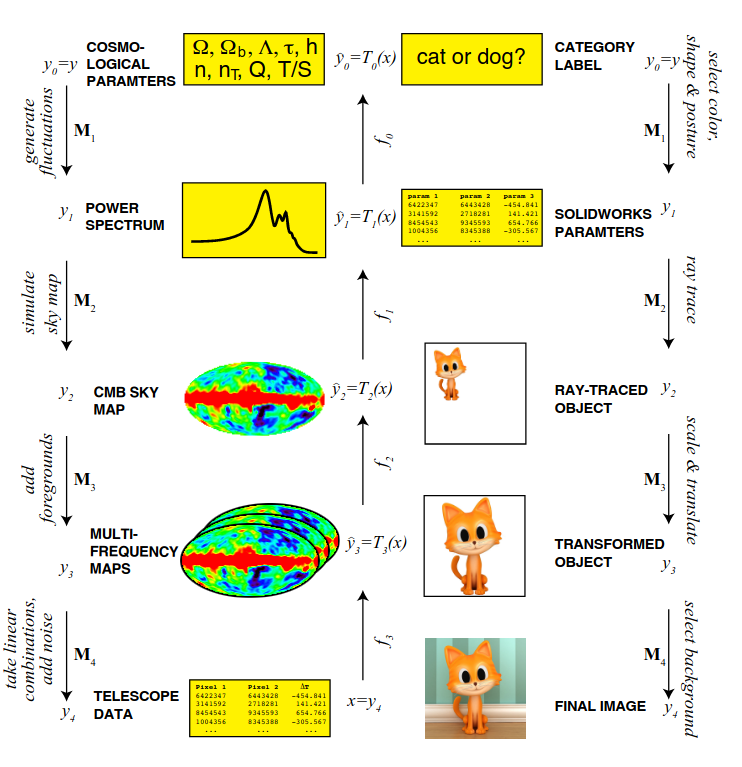
\includegraphics[width=0.6\textwidth]{fig/diagram.png}
        \caption{Diagrama ilustrando a cadeia de processos físicos}
    \end{figure}

\end{frame}

\section{Referências}
\begin{frame}
\tableofcontents[currentsection]
\end{frame}

\begin{frame}
\frametitle{Referências}
\vspace{-2em}
\scriptsize
\bibliographystyle{abntex2-alf}
\bibliography{refs.bib}    
\end{frame}

\begin{frame}

\begin{center}
\Large Obrigado!
\end{center}

\vspace{1em}
Contato: riffel.felipe@grad.ufsc.br 

\vspace{1em}

Repositório com os materiais da apresentação: https://github.com/felipekriffel/Mestrado
    
\end{frame}

\end{document}

